\section{Aufbau und Durchführung}
\label{sec:AufbauUndDurchführung}
\subsection{Aufbau}
\label{sec:Aufbau}
Der grundlegende Aufbau ist in der Abbildung \autoref{fig:Versuchsaufbau} zu erkennen.
Der verwendete Helium-Neon-Laser besteht aus einem Laserrohr, das mit einem Helium-Neon-Gemisch gefüllt ist. An den Enden des Rohrs befinden sich Brewster-Fenster, die eine definierte Polarisation des Laserstrahls ermöglichen. Dahinter sind zwei Resonatorspiegel montiert, wobei einer nahezu vollständig reflektierend ist und der andere teilweise durchlässig, sodass dort die Laserstrahlung austritt. Beide dieser Spiegel haben einen Krümmungsradius von $r = 1400\,\si{\milli\meter\per{\text{flat}}}$. Alle Komponenten sind auf einer optischen Bank befestigt.\\
Ein zusätzlicher Justierlaser mit der Wellenlänge $\lambda = \SI{352}{\nano\meter}$ wird über eine Blende und Umlenkspiegel in den Strahlengang eingeführt, um die Justage zu erleichtern. Der eigentliche Laserstrahl wird je nach Versuchsteil über verschiedene optische Elemente wie Polarisationsfilter, eine Modenblende, ein optisches Gitter oder Linsen geleitet. Die Messung der Intensitätsverteilung erfolgt über einen Detektor, der entlang einer Schiene verschoben werden kann. \cite{anleitungV61}
\begin{figure}
    \centering
    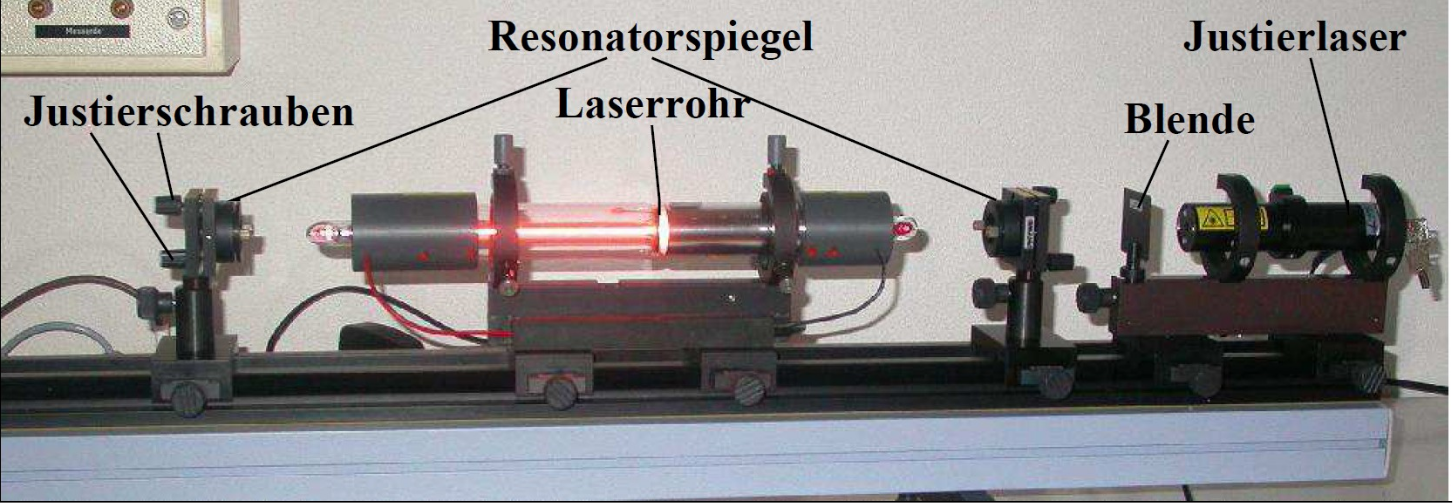
\includegraphics[width=0.75\textwidth]{Bilder/Aufbau.png}
    \caption{Der schematische Aufbau für den He-Ne Laser. \cite{anleitungV61}}
    \label{fig:Versuchsaufbau}
  \end{figure}

\subsection{Durchführung}
\label{sec:Durchführung}
Die folgende Durchführung basiert auf den Angaben aus \cite{anleitungV61}.
Zunächst wird der Strahlengang des He-Ne Lasers mithilfe des Justierlasers und einer Blende eingerichtet. Dabei wird der Justierlaser so ausgerichtet, dass sein Strahl entlang der optischen Achse der Bank verläuft. Über zwei Umlenkspiegel wird der He-Ne Strahl an den Justierstrahl angepasst.\\
\textbf{1. Überprüfen der Stabilitätsbedingung:}\\
Zur Überprüfung der Stabilitätsbedingung des Resonators wird der Abstand zwischen den beiden Spiegeln systematisch verändert und die Stabilitätsbedingung überprüft.
Hierfür muss für jede eingestellte Länge erneut die Justage durchgeführt werden.\\
\textbf{2. Beobachten von TEM-Moden:}\\
In dem Resonator wird als Modenblende ein dünner Wolframdraht mit einem Durchmesser von $d=\SI{0.005}{\milli\meter}$  eingeführt, um die Moden zu stabilisieren.
Zudem wird eine Streulinse verwendet, um die verschiedenen Moden sichtbarer zu machen. 
Die Intensitätsverteilung wird mithilfe eines Detektors in Abhängigkeit Abstände der Maxima $x$ aufgenommen. 
Dies wird für zwei Moden durchgeführt.\\
\textbf{3. Bestimmung der Polarisation:}\\
Zur Untersuchung der Polarisation wird ein Polarisator in den Strahlengang eingebracht. Anschließend wird dieser schrittweise um jeweils $\SI{5}{\degree}$ gedreht, während die Intensität hinter dem Polarisator mit einer Photodiode aufgenommen wird.\\
\textbf{4. Multimodenbetrieb und Frequenzspektrum des Lasers:}\\
Zur Untersuchung des Frequenzspektrums des Lasers im Multimodebetrieb wird der Laserstrahl auf eine Photodiode mit einer Bandbreite von \SI{1}{\giga\hertz} geführt. 
Das elektrische Signal wird anschließend mit einem Spektrumanalysator ausgewertet. Dabei wird der Resonatorabstand $L$ variiert, und für jede Einstellung werden die Frequenzen der beobachteten Peaks aufgenommen. Dadurch lässt sich der Modenabstand bestimmen und die Anzahl gleichzeitig verstärkter longitudinaler Moden analysieren.\\
\textbf{5. Beugung am Gitter und Bestimmung der Wellenlänge:}\\
Zur Bestimmung der Wellenlänge wird ein optisches Gitter senkrecht zum Strahl positioniert. Die Beugungsmaxima werden auf einem Schirm sichtbar gemacht. Der Abstand zwischen den Maxima wird gemessen, ebenso wie der Abstand zum Gitter.\\